% !TeX root = ../main.tex
% Add the above to each chapter to make compiling the PDF easier in some editors.

\chapter{Related Work}\label{chapter:relatedWork}
The optimization of queries is a pivotal aspect in the realm of database performance profiling, and various existing approaches are dedicated to supporting this field with visualization tools. This chapter offers an overview about the existing work in the domain of the visualization of database performance profiling.
We will investigate the importance of optimizing query executions in database systems and the role of visualizations in identifying potential improvements.
As performant measurement and analysis play a crucial role in developing and optimizing database systems, 
it is essential to examine the state-of-the-art techniques and tools that have been used in this domain.
We will also cover a visualization tool closely associated with this thesis, as its key feature is integrated into our tool, the Benchy Viewer.


\section{Database Performance Profiling }

Performance profiling in database systems is crucial for optimizing their execution regarding achieving optimal hardware utilization and query efficiency.
Profiling the performance of database systems involves collecting and analyzing various performance metrics during query execution.
\\Besides profilers presenting results at the instruction and function granularity, a paper on "Profiling Dataflow Systems on Multiple Abstraction Levels" \cite{profiling-dataflow} proposes a solution that tracks the code generation process and aggregates profiling data to higher abstraction levels. This approach helps bridging the semantic gap between low-level profiles and high-level constructs, making it easier for developers to interpret profiling results and identify bottlenecks and hotspots in the system. The paper introduces the concept of Tailored Profiling, which extends the compilation steps to annotate the generated code with metadata. This enables the mapping of profiling results back to desired abstraction levels and provides more understandable profiling data.
Building on the insights from this work, the opportunity arises to create more meaningful visualizations regarding the dataflow in system performance profiling.
\\ An essential concept of this thesis is to develop and provide effective performance visualizations built upon the concepts of tailored profiling, which should contribute to a better understanding of the system's performance and support the location of potential optimization possibilities. 
Thus, we integrate an intuitive and interactive visualization tool that is able to break down complex queries into their constituent operators and pipelines. We clarify further details about the implementation in Chapter~\ref{chapter:implementation}.

\section{Related visualization tools}

This section explores related visualization tools that aid developers analyse their database system queries, with a specific focus on performance visualization. We will go through the Query Plan Difference Visualiser \parencite*{semantic-diff} and the Umbra Profiler \parencite*{profiling-dataflow}, which are both tools, that are strongly related to the Benchy Viewer. 


\subsection{Query Plan Difference Visualiser}
\label{subsec:semantic-diff}

The efficiency of a database system's query execution relies on the execution plan it generates.  Given the complexity of finding the best plan, the comparison of query plans both within a single system and accross different systems has garnered attention. This comparative analysis aims to gain valuable insights and identify potential optimisation opportunities.

\begin{figure}[h]
  \centering
  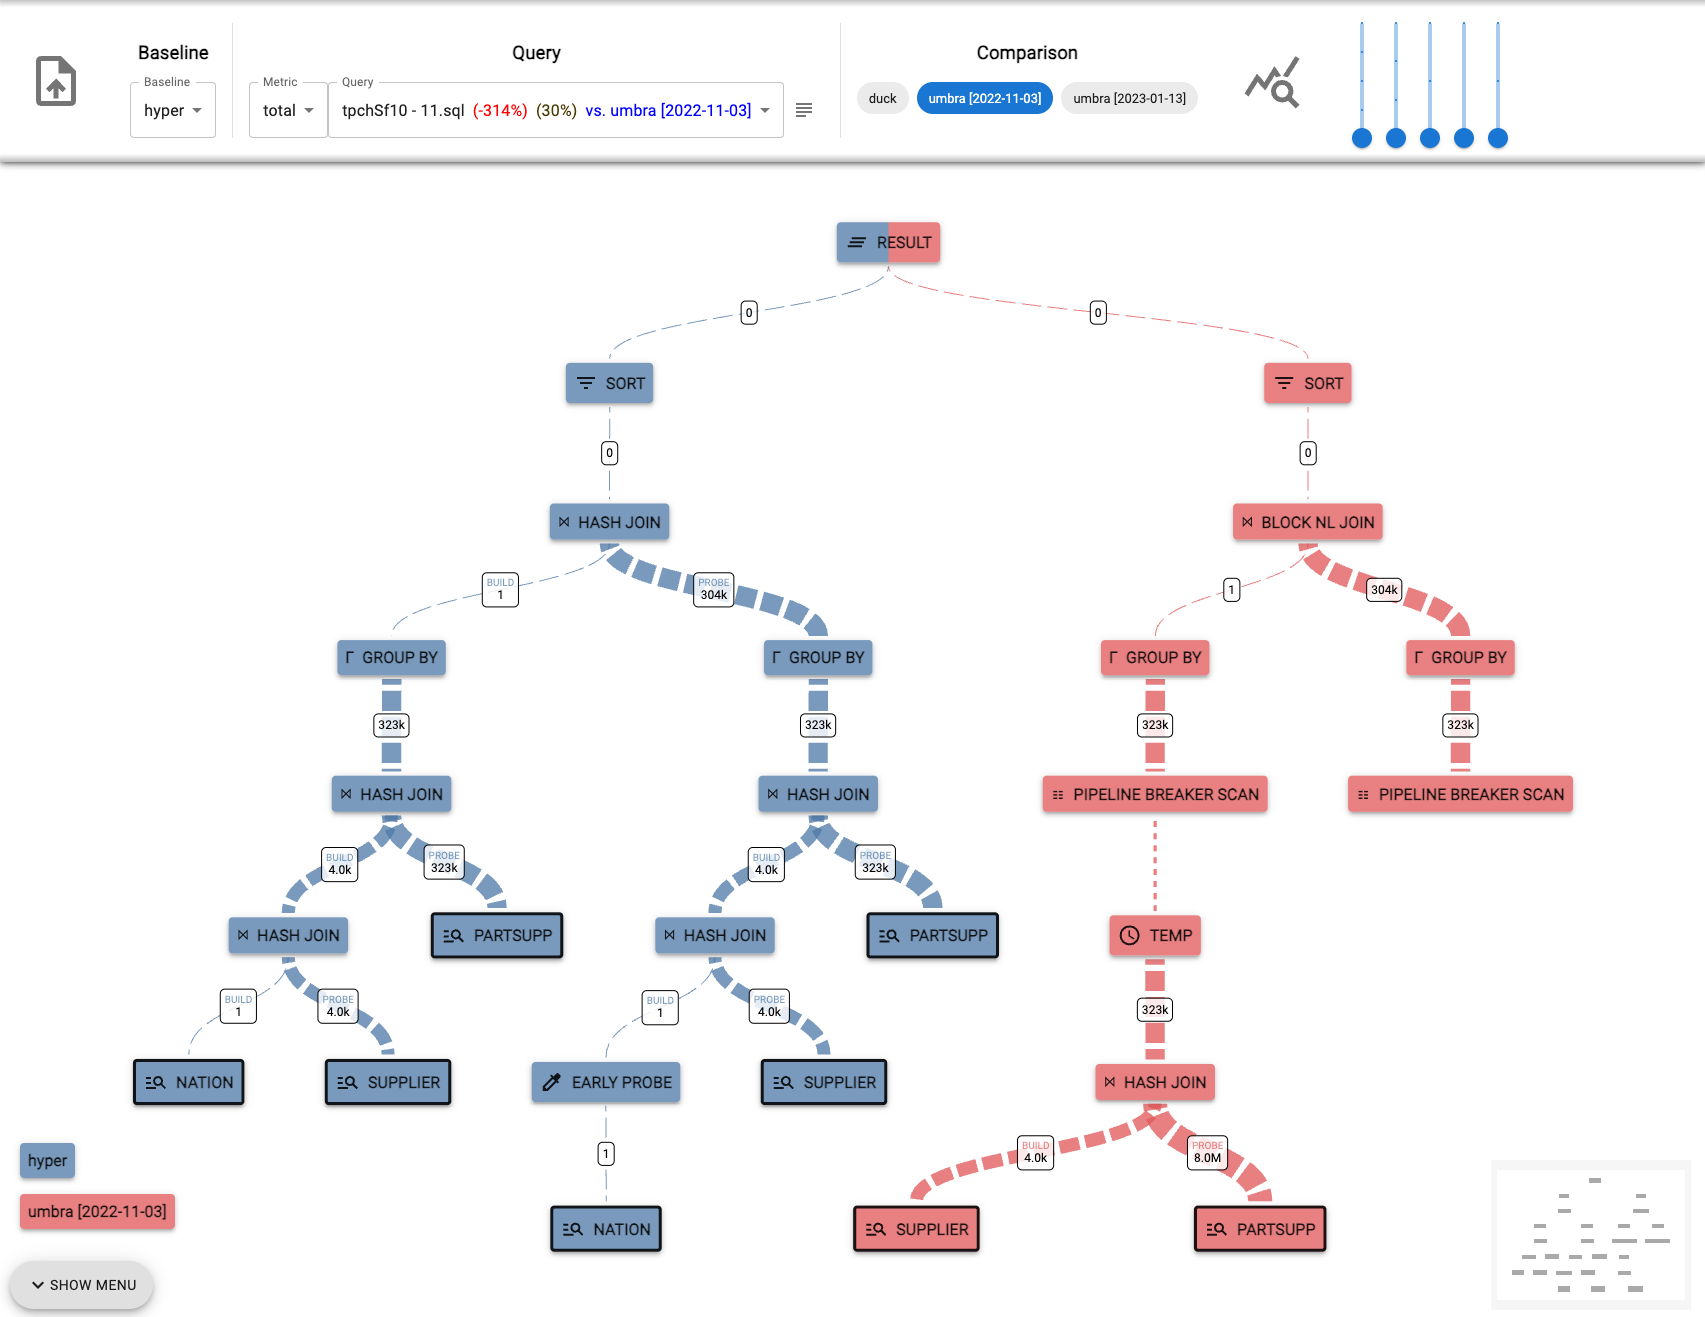
\includegraphics[width=0.8\linewidth]{figures/semantic-diff.png}
  \caption{Query Plan Difference Visualiser.}
  \label{fig:semantic-diff}
\end{figure}

Query execution plans describe the step-by-step hierarchical sequence of physical operations that a database system uses to process a particular SQL query. The fascinating aspect of this is that identical queries can result in different plans when processed by different database systems. This variability in plan generation can have a significant impact on overall performance \parencite*{GroupjoinAndNestedAggregates}.
\\The Query Plan Difference Visualiser is a web application that compares and visualises these physical query execution plans from different relational database systems, as shown in Figure~\ref{fig:semantic-diff}. It is designed for database developers who want to inspect the correlation between variations in query execution speed and the respective query plans. Through enhanced hierarchical differencing algorithms with semantic information about query plans, the tool is able to interactively capture and present  the difference between query plans. This is particularly useful for comparing different database systems or different versions of the same system when varying query plans are used by the systems under test to process the same query. Furthermore, it provides the flexibility to pick an arbitrary number of systems for which to compare plans and select a metric for evaluating query performance, such as total runtime or compilation time. For the given metric, it directly shows the difference between the baseline system and the better system.
\\ Once a query plan is initialized, the comparative tool provides the option to improve the clarity of the query plan visualization using various configuration settings. For instance, the tool offers a match mode selection, allowing users to capture the tree from, e.g., a top-down or bottom-up matching perspective. With the Expand and Collapse feature, users can collapse entire subtrees and selectively expand specific child nodes, customizing the focus of the visualization and tailoring the area of attention to the most interesting parts of the tree.
For query plans containing Directed Acyclic Graph (DAG) edges, such as the Pipeline Breaker Scan operator in Umbra, the tool offers support to include these DAG edges and consider them during the matching process. Additionally, to enable more effective comparisons against systems that generate non-DAG-shaped plans, an option is available to replicate subtrees instead.
\\ Database developers often find value in comparing query plans with other systems, particularly when they have thoroughly examined different results using quantitative metrics and cardinality estimates. 
Therefore, we decided to integrate the Query Plan Difference Visualiser with its core features of comparing query plans. In addition to visualising quantitative metrics from different database systems within the Benchy Viewer, the incorporation of the Query Plan Difference Visualiser with its capabillities will further enhance our objective of simplifying the detection of performance bottlenecks in query execution and optimizing database systems.

Hence, the Query Plan Difference Visualiser is strongly related to this thesis and we will dive deeper into the integration of the comparative tool in \ref{sec:semantic-diff-integration}.



\subsection{Umbra Profiler}
The Umbra Profiler \parencite*{umbra-profiler-schott,umbra-profiler-schworm} enables in-depth analysis for identifying bottlenecks in query execution processes of the database system Umbra.
\\ It is integrated with a backend application for preparing extensive profiling data and offers multiple perspectives, including a runtime dashboard, a memory dashboard, and an instruction dashboard, each depicting distinct information, as illustrated in Figure~\ref{fig:umbra-profiler}.

\begin{figure}[h]
  \vspace{0.5cm}
  \centering
  \begin{subfigure}[b]{0.3\linewidth}
    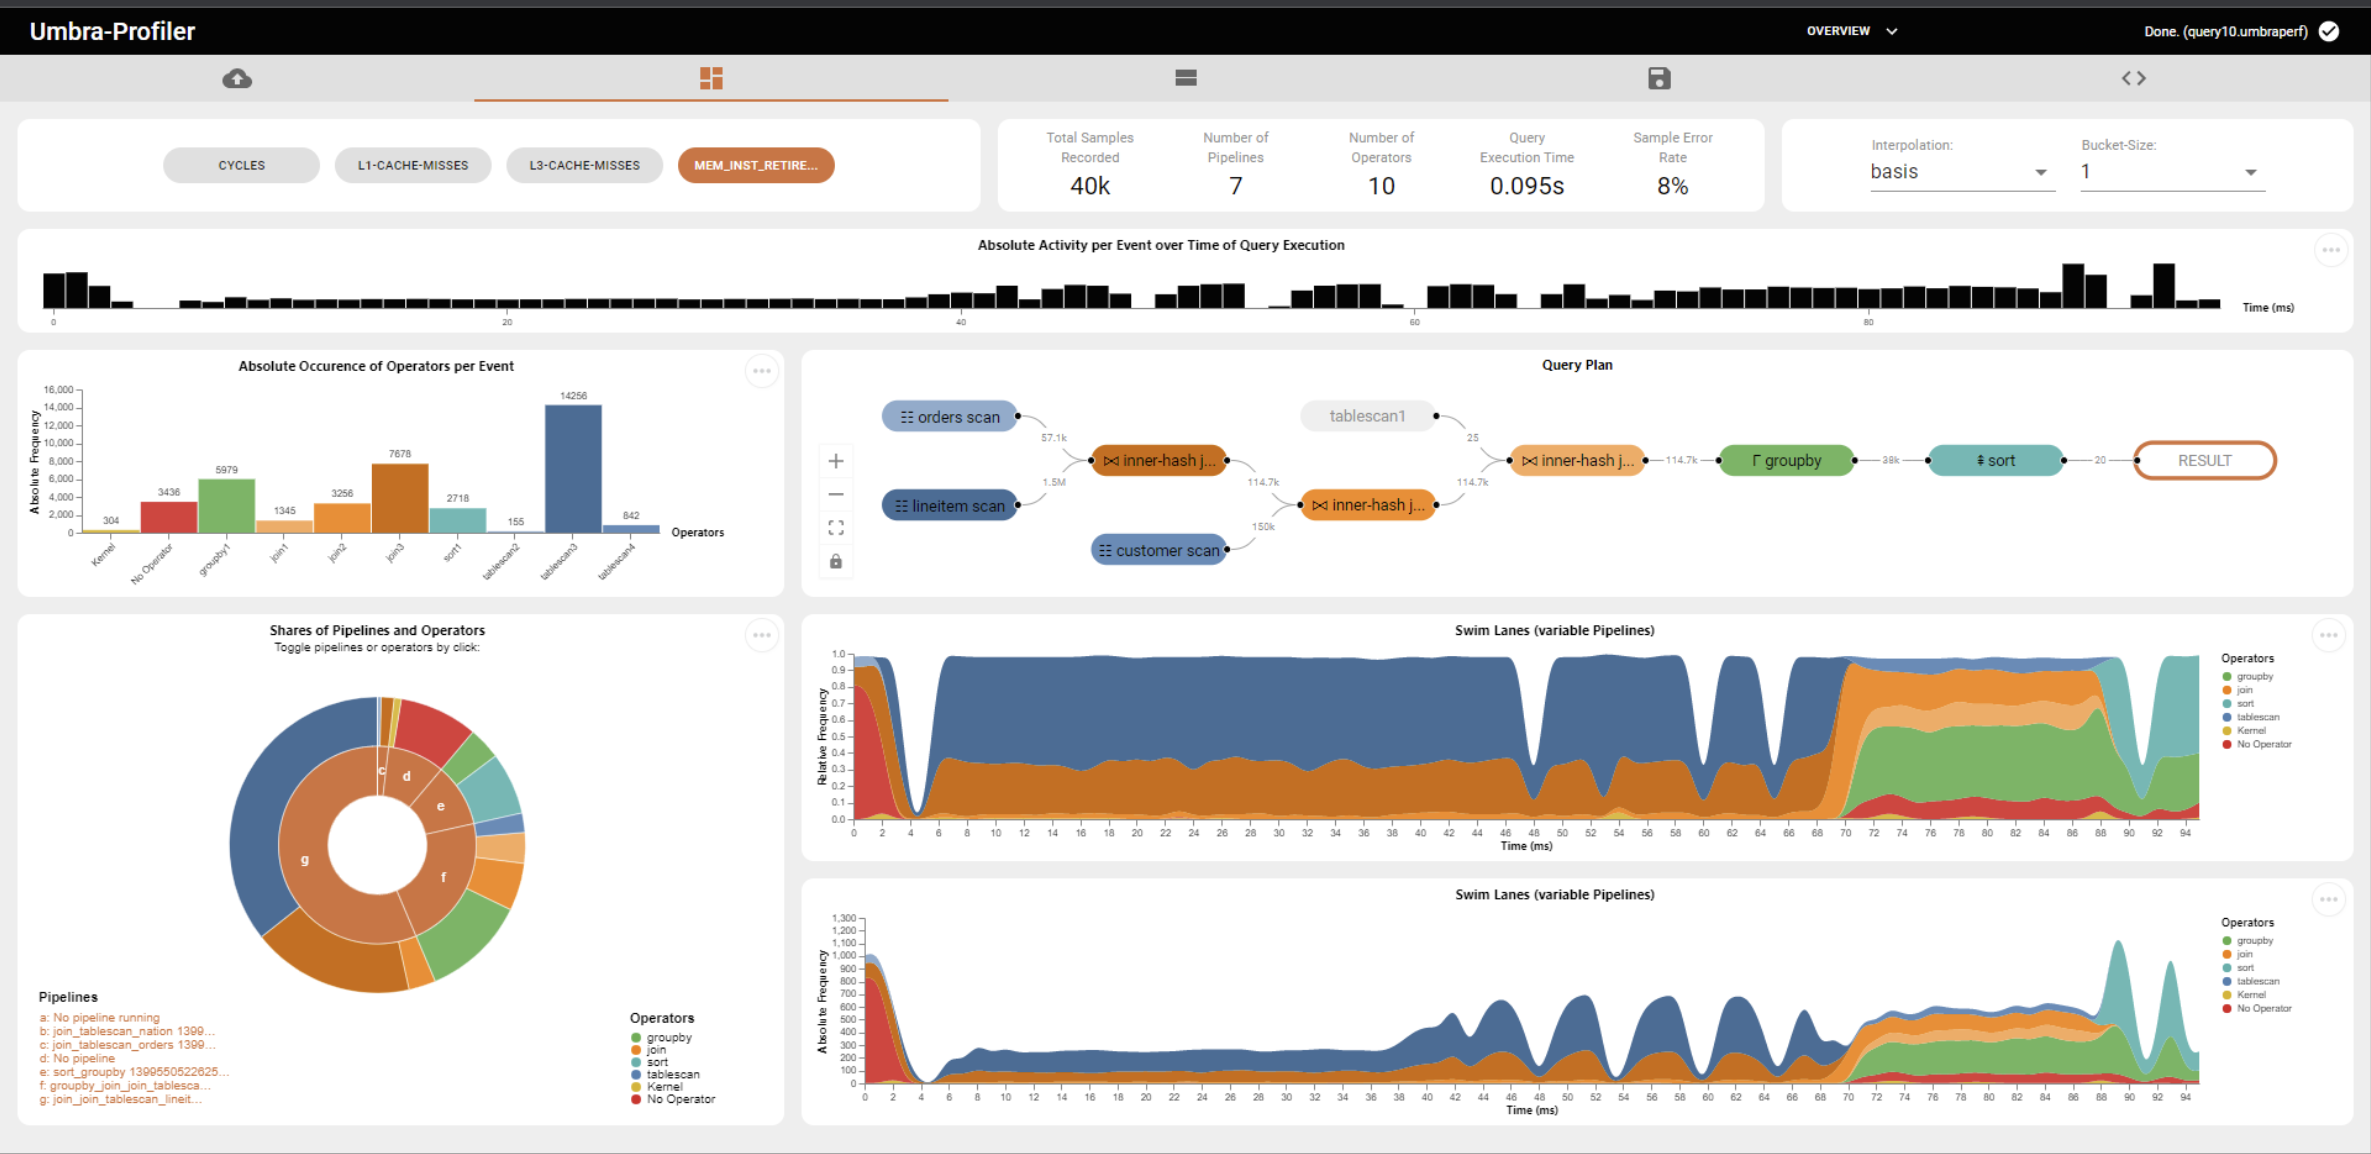
\includegraphics[width=\linewidth]{figures/umbra-profiler-runtime-dashboard.png}
    \caption{Runtime Dashboard.}
      \label{fig:umbra-profiler-runtime-dashboard}
  \end{subfigure}
  \hspace{0.5cm} % Adjust the horizontal space between the figures
  \begin{subfigure}[b]{0.3\linewidth}
    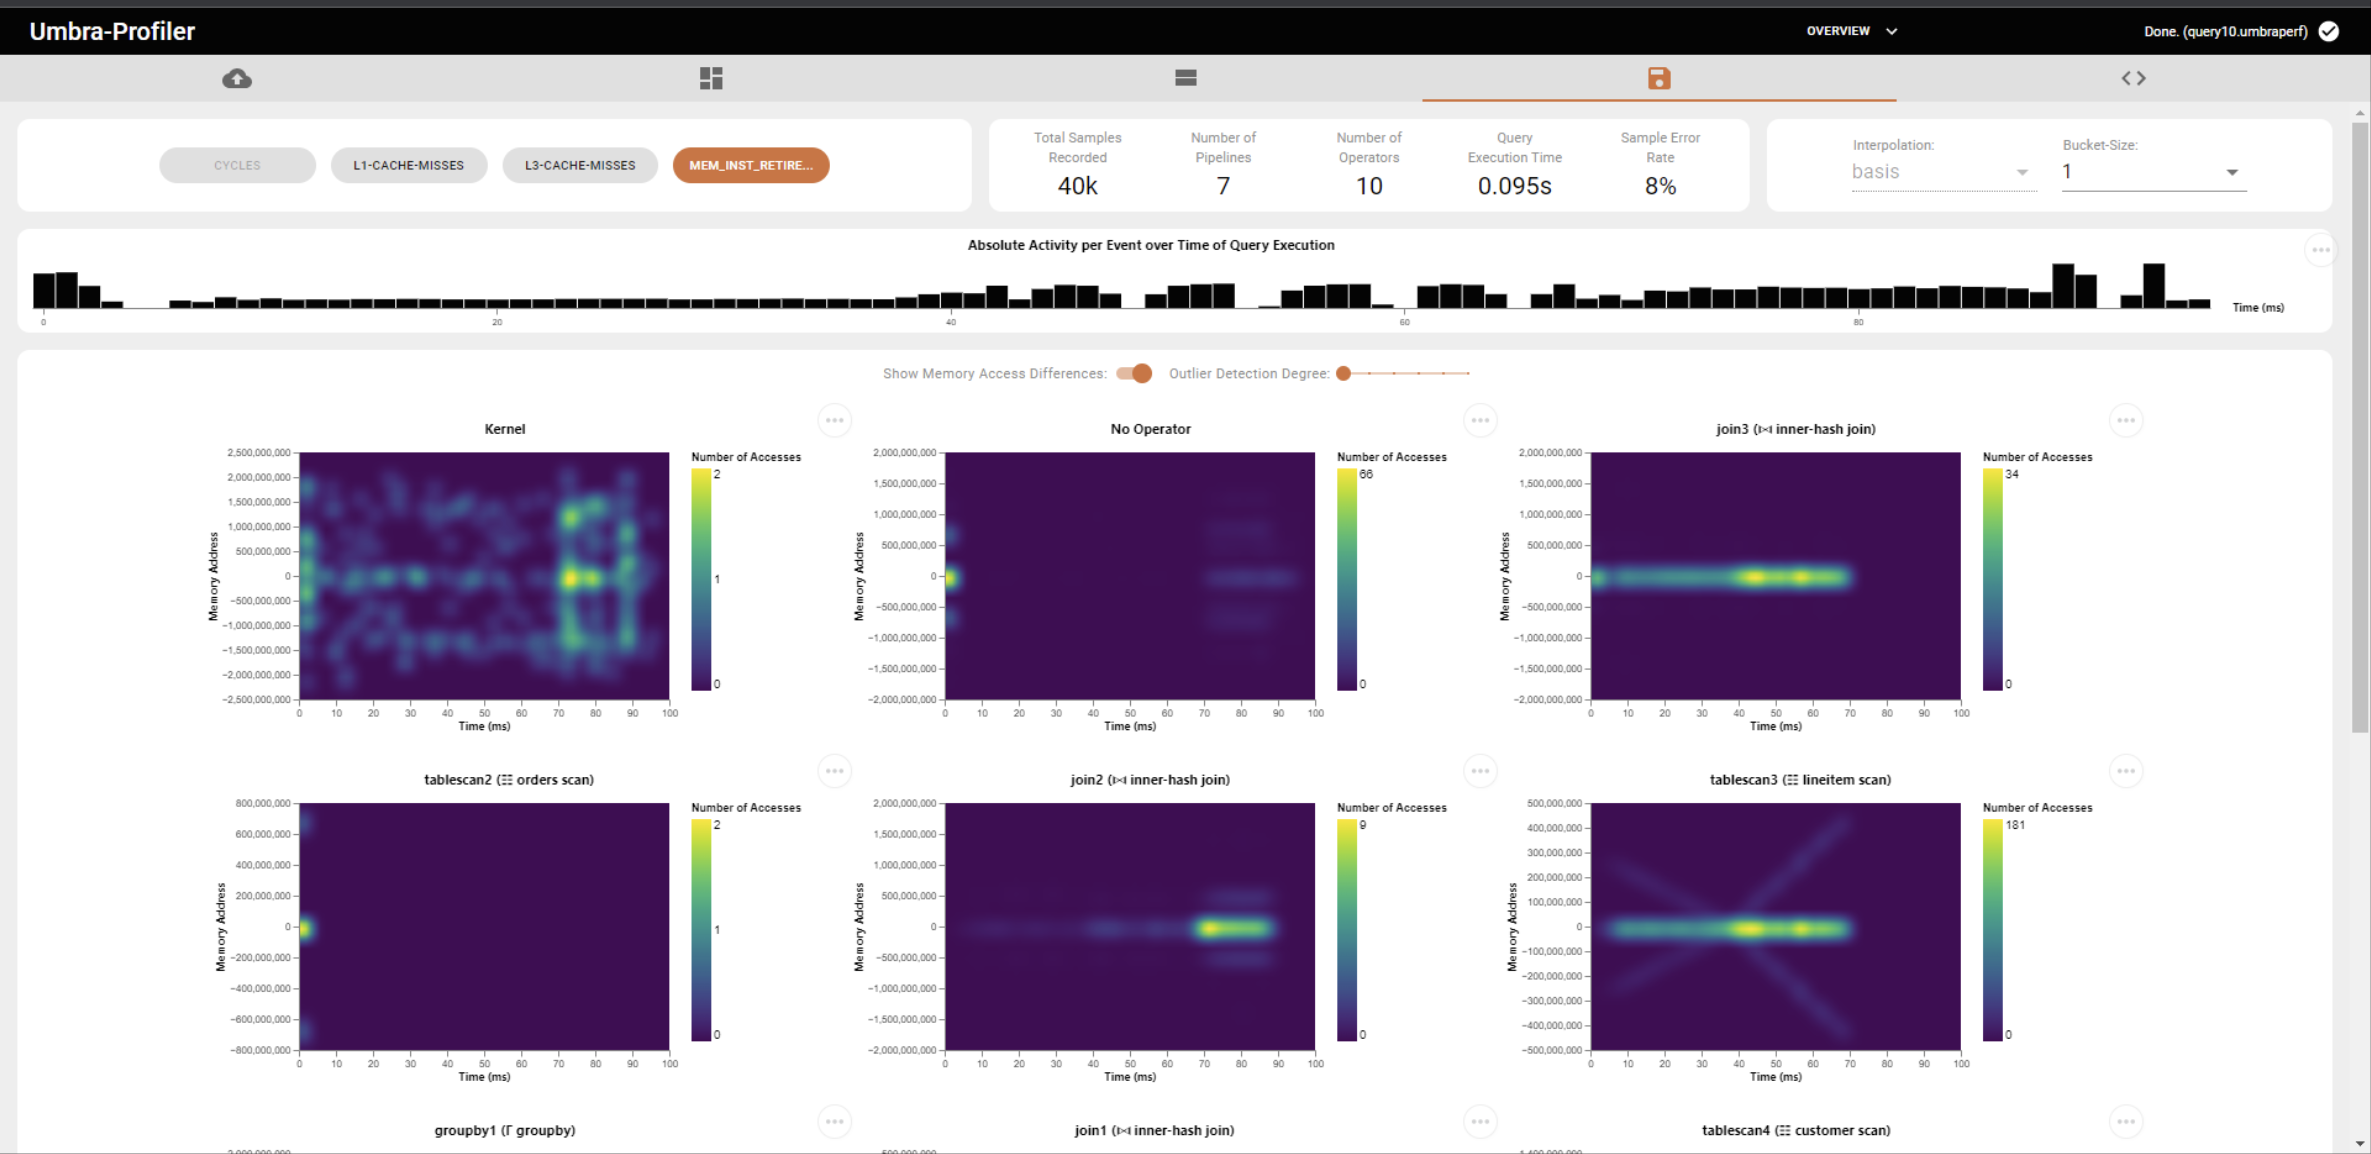
\includegraphics[width=\linewidth]{figures/umbra-profiler-memory-dashboard.png}
    \caption{Memory Dashboard.}
      \label{fig:umbra-profiler-memory-dashboard}
  \end{subfigure}
  \hspace{0.5cm} % Adjust the horizontal space between the figures
  \begin{subfigure}[b]{0.3\linewidth}
    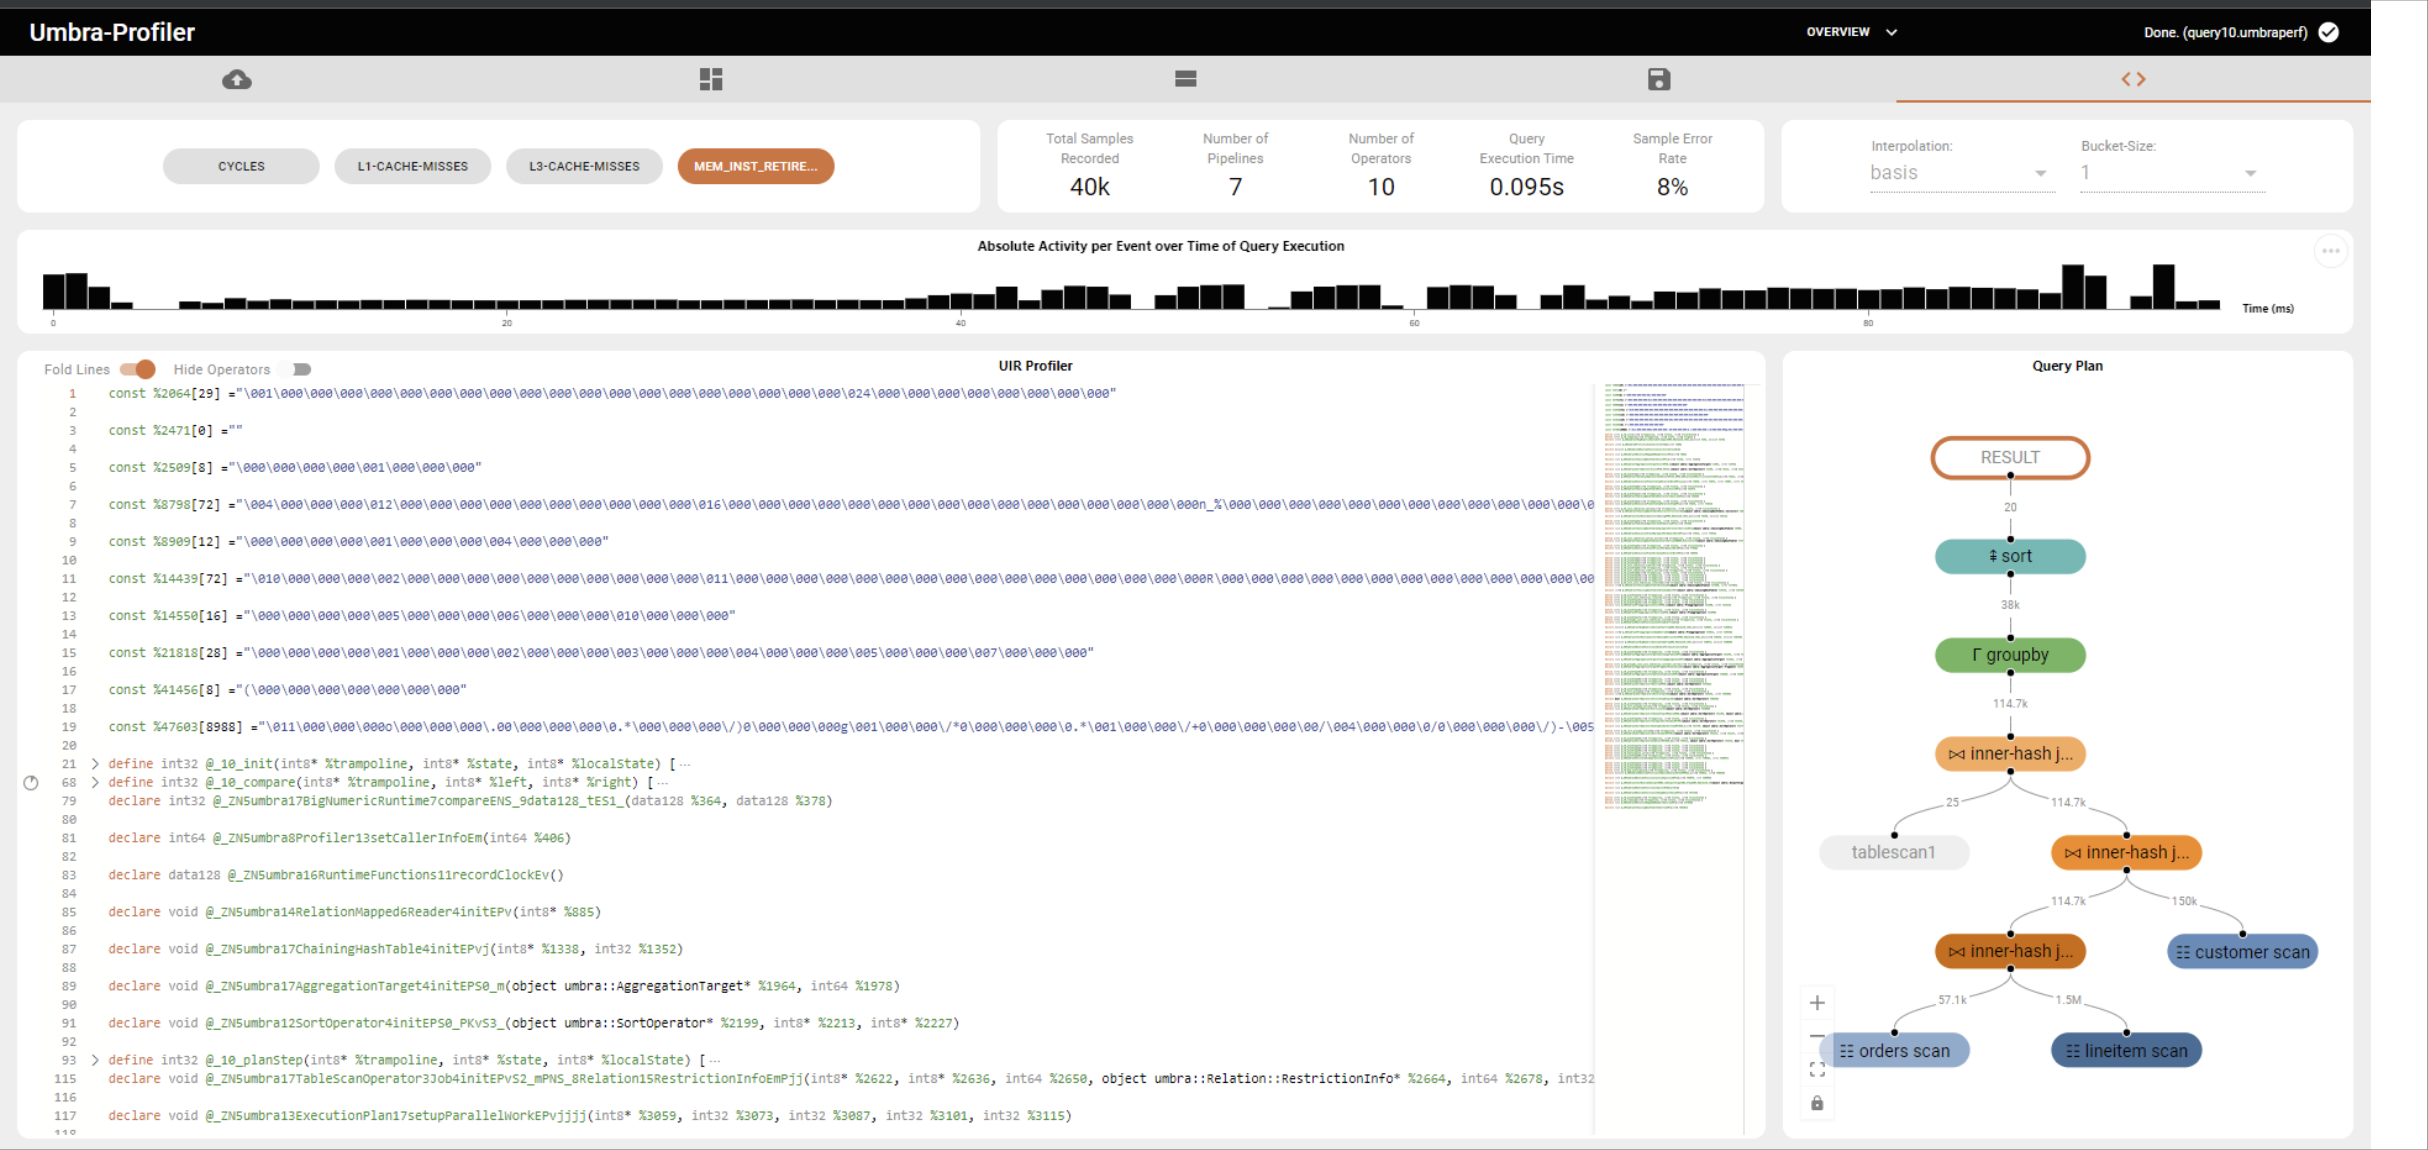
\includegraphics[width=\linewidth]{figures/umbra-profiler-instruction-dashboard.png}
    \caption{Instruction Dashboard.}
      \label{fig:umbra-profiler-instruction-dashboard}
  \end{subfigure}
  \caption{Umbra-Profiler: A tool for analyzing and profiling Umbra’s compiling
  queries.}
  \label{fig:umbra-profiler}
\end{figure}

The runtime dashboard is the default view that appears after providing recorded hardware samples of a query execution. It offers an initial overview of the query execution structure, allowing users to analyze the activity of specific processor events, operators, and pipelines over time. Abnormalities in execution, such as resource-intensive operations, can be identified, aided by visualizations including key performance indicators, activity histograms, bar charts, query plans, sunburst charts, and swim lanes.
\\The memory behavior dashboard focuses on memory access patterns in query execution. It offers memory heatmaps for each operator, showing either absolute memory accesses or sequential memory address differences.
\\The instruction Dashboard facilitates detailed analysis of query execution using Umbra Intermediate Representation (UIR) \parencite*{Kersten2021TidyTA} instructions. It allows comparison of UIR instructions with query plans to identify performance problems based on costs and occurrences. 
\\Similar to the Benchy Viewer, the goal is to support database engineers in optimizing query execution by providing an interactive user interface, enabling an effective in-depth analysis process. 
\\The Umbra Profiler is designed based on the innovative Tailored Profiling approach \cite{profiling-dataflow}, where the connection between query plans and compiled code is maintained.
\\However, unlike the Benchy Viewer, the Umbra Profiler is focused to operate exclusively with the database system Umbra. In contrast, the Benchy Viewer has the versatility to function with multiple database systems or multiple instances of a single database system.
\\In broad terms, the Umbra Profiler is primarily designed for in-depth analysis of query performance within a single database system, while the Benchy Viewer is oriented towards its comparative function, enabling the comparison of queries executed by different instances. This comparative approach is the main essence  of the concept of the Benchy Viewer, which aims to enhance the understanding of differences between database instances.

An effective scenario that synergizes the Benchy Viewer and the Umbra Profiler would involve identifying intriguing queries using the Benchy Viewer and subsequently conducting comprehensive analyses using the Umbra Profiler.


